\section{RQ1: Statistical Analysis of Profile Coherence}
\label{sec:rq1}

RQ1 establishes the diagnostic axis of the paper. It asks how prevalent profile-discordance is in observed FAR-Trans Buy transactions, whether it is a stable customer trait or transaction-level noise, and whether it carries an economic penalty once asset volatility, customer segment, and year are controlled for. We first define the risk bands and the asset risk-band assignment the entire paper relies on, formalise the Profile Coherence metric, describe the dataset, then present the diagnostic analysis and the return-premium regression in turn.

\subsection{Risk Bands}
\label{sec:setup:bandassignment}

\subsubsection{Ordinal band scale}
Customers and assets share the same 4-point ordinal scale running from Conservative to Income to Balanced to Aggressive, encoded 0 to 3. The customer band $b_u$ is taken from FAR-Trans's \texttt{riskLevel} field. FAR-Trans provides both declared values and regression-imputed \texttt{Predicted\_*} entries, and both are mapped to the same ordinal scale. Customers whose entry is \texttt{Not\_Available} or missing are excluded from all coherence computations. The asset band $b_i$ is assigned by the three-step hierarchical rule below, applied in order.

\subsubsection{Step 1: subcategory metadata} Mutual funds are labelled directly from their subcategory: Money Market funds are treated as Conservative, Bond funds as Income, Balanced as Balanced, and Equity or Large Cap as Aggressive. Bond instruments are labelled by issuer type: Government as Conservative, Corporate as Income, and any remaining bond subcategory as Income by default.

\subsubsection{Step 2: volatility quartiles for stocks} Stocks carry no subcategory tag we can use, so they fall through to a volatility rule. For each ISIN we compute the annualised standard deviation of daily log returns on a trailing 252-day window, then bucket all stocks into the four bands by the stock-only quartile thresholds $(q_1, q_2, q_3)$.

\subsubsection{Step 3: residual default} Any asset that falls through both prior steps is assigned to Balanced.

Applying the three steps above produces an asset-band distribution of $(190, 333, 105, 178)$ across (Conservative, Income, Balanced, Aggressive) over $|A| = 806$ assets, which feeds the band-conditional random baseline $\pi(b)$.

\subsection{Profile Coherence}
\label{sec:method:pck}

\subsubsection{Pairwise discordance}
\begin{equation}
d(u, i) = |b_u - b_i| \in \{0, 1, 2, 3\}.
\end{equation}
A recommendation is \emph{profile-coherent} iff $d \leq 1$. We adopt this $\pm 1$ band tolerance by design, to mirror MiFID II's adjacency allowance for borderline suitability rather than to penalise every single-band drift as a violation.

\subsubsection{Aggregation}
\begin{equation}
\text{PC@}k(u) = \frac{1}{k} \left|\{ i \in \text{top}_k(u) : d(u, i) \leq 1 \}\right|.
\end{equation}
Two implementation rules complete the definition. First, recommenders returning fewer than $k$ items use the actual number of items returned as the denominator. Second, customers with no assigned risk band ($b_u = \emptyset$) are dropped from the aggregate. Per-split PC@$k$ is the unweighted mean across eligible customers and the headline numerics average over all splits.

\subsubsection{Band-conditional random baseline}
The closed-form expectation of PC@$k$ under a uniformly random recommender for band $b$ is given by
\begin{equation}
\pi(b) = \frac{|\{ i \in A : |b - b_i| \leq 1 \}|}{|A|},
\end{equation}
where $A$ is the asset universe. With the asset-band distribution from Section~\ref{sec:setup:bandassignment}, this yields $\pi(b) = (0.65, 0.78, 0.76, 0.35)$.

\subsubsection{PC-lift@$k$}
Per-user PC@$k$ is normalised against the random reference at the customer's own band:
\begin{equation}
\text{PC-lift@}k(u) = \frac{\text{PC@}k(u)}{\pi(b_u)}.
\end{equation}
Lift $> 1$ beats the band-conditional random rate, while lift $= 1$ matches it. Because 77.9\% of FAR-Trans assets sit in the Conservative, Income, and Balanced bands, a recommender that pushes Income assets at everyone would score well on raw PC@$k$ for any user whose tolerance set includes Income. Dividing by $\pi(b_u)$ removes this advantage, so bands that are easier to satisfy by chance are not credited for it and the lift values can be compared across bands.

\subsection{Dataset}
\label{sec:setup:dataset}

In addition to what was introduced in Section~\ref{sec:intro}, FAR-Trans~\cite{sanzcruzado2024fartransinvestmentdatasetfinancial} provides 159{,}135 Sell transactions. Of the 29{,}090 customers, 28{,}770 (98.9\%) carry a declared or regression-imputed MiFID II risk band, and the remaining 320 are excluded from all coherence computations. Customer profiles also include \texttt{customerType} and \texttt{investmentCapacity}, both of which enter our regression study later as controls.

\subsection{Prevalence and Structure of Discordance}
\label{sec:rq1:prevalence}

We characterise discordance in four slices, starting from the pooled transaction rate and drilling into the customer, band, and year dimensions in turn. At the transaction level (Figure~\ref{fig:rq1-dist}), of 228{,}241 scoreable Buys:
\begin{enumerate}
    \item 18.6\% violate the declared band by two or more steps.
    \item 81.4\% are coherent, of which 34.1\% are strictly coherent ($d = 0$).
    \item Mean discordance is 0.874 bands across all scoreable Buys, indicating that when mismatches occur they are usually around a single band step.
\end{enumerate}

All in all, nearly one in five scoreable Buys lands two or more bands away from the customer's declared tolerance. That violation rate is too large to dismiss as sampling noise, and it is the empirical motivation for treating profile coherence as a measurable evaluation axis rather than a property the baselines can be assumed to satisfy.

\begin{figure}[H]
    \centering
    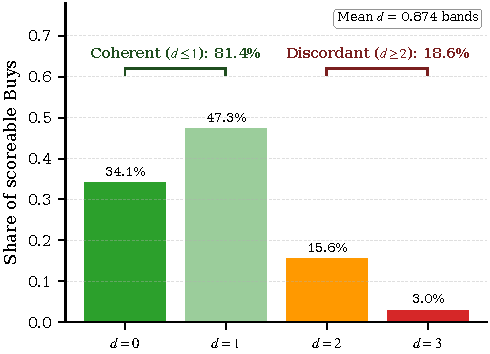
\includegraphics[width=\linewidth]{figures/discordance_distribution.pdf}
    \caption{Distribution of pairwise discordance $d$ over 228{,}241 scoreable Buys. Most mass sits at $d \leq 1$ (coherent), with non-negligible density at $d \geq 2$ (discordant).}
    \label{fig:rq1-dist}
\end{figure}

The pooled rate cannot tell us whether these violations are i.i.d.\ transaction-level slips spread thinly across the customer base or a structural trait concentrated in a subset. Slicing by customer settles the question. The per-customer discordant share (Figure~\ref{fig:rq1-self}) is sharply bimodal, concentrating in the lowest and highest bins rather than clustering near the 18.6\% population mean. More explicitly, 64.4\% of banded customers are fully coherent across every Buy and 17.2\% are fully discordant.

\begin{figure}[H]
    \centering
    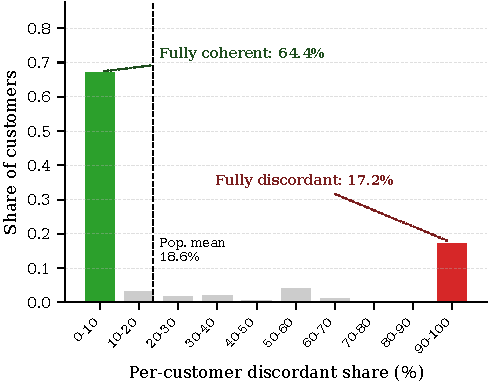
\includegraphics[width=\linewidth]{figures/self_discordance.pdf}
    \caption{Per-customer share of discordant Buys is sharply bimodal, concentrating in the lowest and highest bins and ruling out i.i.d.\ transaction-level noise.}
    \label{fig:rq1-self}
\end{figure}

Hartigan's dip test on the 28{,}770 per-customer values rejects unimodality ($D = 0.086$, $p < 10^{-15}$), confirming that discordance is a persistent customer-level trait rather than i.i.d.\ transaction-level noise.

Since the trait is customer-level, the next question is which customers carry it. Coherence per declared band is U-shaped (Figure~\ref{fig:rq1-per-band}). The two centre bands sit around 90\%, while Conservative drops to 45.1\% (possibly reflecting a ``reach for yield'' tendency) and Aggressive to 56.2\% (possibly reflecting a regression toward safer assets). This concentration of mismatch at the ordinal extremes corroborates the bimodality finding from the customer slice.

\begin{figure}[H]
    \centering
    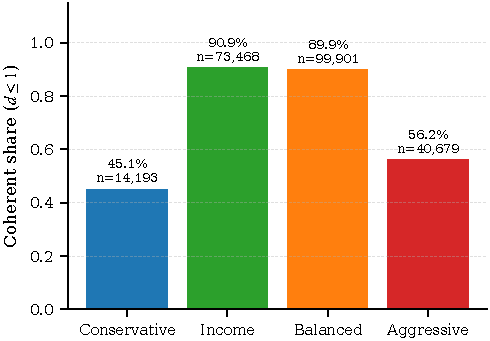
\includegraphics[width=\linewidth]{figures/per_band_coherence.pdf}
    \caption{Coherence share by declared band. The U-shape supports the bimodality result of Figure~\ref{fig:rq1-self}: discordance concentrates on the ordinal extremes.}
    \label{fig:rq1-per-band}
\end{figure}

A final slice rules out a regime-driven artefact. Mean discordance is flat across 2019 to 2022 (within 0.02 bands, see Figure~\ref{fig:rq1-yearly}), so the pattern is not the product of any single year's market conditions. The 2018 value (0.98) sits higher but covers a small slice. MiFID II came into force on 2018-01-03, the exact start of FAR-Trans, so we hypothesise the elevation as a transition effect. However, this hypothesis is not tested and is potential future work.

\begin{figure}[H]
    \centering
    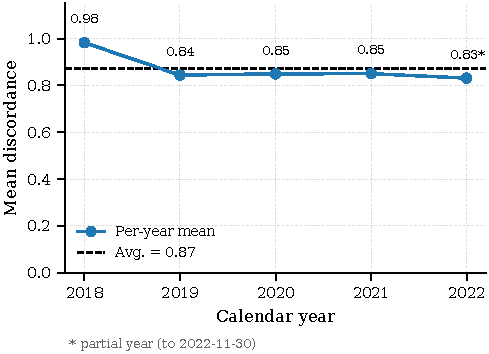
\includegraphics[width=\linewidth]{figures/yearly_discordance.pdf}
    \caption{Mean discordance by calendar year. The 2019 to 2022 cluster sits within 0.02 bands, with 2018 elevated (transition-effect hypothesis).}
    \label{fig:rq1-yearly}
\end{figure}

\begin{table*}[!t]
\centering
\small
\begin{tabular}{lrrrr}
\toprule
Term & Estimate & Std.\ Error & 95\% CI & $p$ \\
\midrule
Intercept                                & $-0.0471$ & $0.0141$ & $[-0.0746,\, -0.0195]$ & $8.1 \times 10^{-4}$ \\
\texttt{is\_coherent}                    & $+0.0294$ & $0.0040$ & $[+0.0215,\, +0.0372]$ & $2.3 \times 10^{-13}$ \\
\texttt{asset\_volatility}               & $-0.1025$ & $0.0165$ & $[-0.1349,\, -0.0701]$ & $5.5 \times 10^{-10}$ \\
\texttt{C(customer\_type)[Legal Entity]} & $+0.0154$ & $0.0486$ & $[-0.0798,\, +0.1106]$ & $0.751$ \\
\texttt{C(customer\_type)[Mass]}         & $+0.0011$ & $0.0132$ & $[-0.0248,\, +0.0269]$ & $0.936$ \\
\texttt{C(customer\_type)[Premium]}      & $+0.0058$ & $0.0135$ & $[-0.0206,\, +0.0322]$ & $0.667$ \\
\texttt{C(customer\_type)[Professional]} & $+0.0247$ & $0.0169$ & $[-0.0084,\, +0.0578]$ & $0.143$ \\
\texttt{C(year)[2019]}                   & $+0.1759$ & $0.0129$ & $[+0.1507,\, +0.2012]$ & $1.4 \times 10^{-42}$ \\
\texttt{C(year)[2020]}                   & $+0.2107$ & $0.0061$ & $[+0.1986,\, +0.2227]$ & $6.2 \times 10^{-259}$ \\
\texttt{C(year)[2021]}                   & $+0.0754$ & $0.0053$ & $[+0.0651,\, +0.0858]$ & $4.1 \times 10^{-46}$ \\
\texttt{C(year)[2022]}                   & $-0.0195$ & $0.0045$ & $[-0.0283,\, -0.0107]$ & $1.4 \times 10^{-5}$ \\
\bottomrule
\end{tabular}
\caption{Full RQ1 OLS coefficient table on 208{,}029 priced Buys, cluster-robust SE on \texttt{customerID}. Reference cell: Inactive \texttt{customerType} (the alphabetically first segment in FAR-Trans), year 2018, $\texttt{asset\_volatility} = 0$, $\texttt{is\_coherent} = 0$.}
\label{tab:rq2-full}
\end{table*}

\subsection{Conditional Return Premium}
\label{sec:rq1:return}

We have shown that discordance is a persistent customer-level trait concentrated at the ordinal extremes. The next question is whether it carries an economic cost: do discordant Buys earn lower returns than coherent ones?

\subsubsection{Regression specification}
We test whether profile-coherent Buys earn different realised returns from discordant ones via a transaction-level Ordinary Least Squares (OLS) regression on 208{,}029 priced Buys with cluster-robust standard errors on \texttt{customerID} and a two-sided Wald test at $\alpha = 0.05$. Clustering is warranted because each customer contributes roughly 8 Buys on average, so within-customer residuals share unobserved shocks. The specification is:
\begin{equation}
\label{eq:rq2-ols}
\begin{split}
r ={}& \beta_0 + \beta_1 \cdot \text{is\_coherent} \\
    &{}+ \beta_2 \cdot \text{asset\_volatility} \\
    &{}+ \mathbf{C}(\text{type})\boldsymbol{\gamma} \\
    &{}+ \mathbf{C}(\text{year})\boldsymbol{\delta} \\
    &{}+ \varepsilon,
\end{split}
\end{equation}
where $r = (p_{\text{end}} - p_{\text{start}})/p_{\text{start}}$ is the 6-month realised return as a decimal fraction (e.g., $r = 0.03$ means a 3 percentage-point gain) and \texttt{is\_coherent} is binary ($d \leq 1$).

Prices are matched via a backward-nearest join: the start price is the most recent close on or before the trade date, and the end price is the most recent close on or before the date six months later. Transactions without a price match within 7 days at either endpoint are dropped. The coefficient of interest is $\beta_1$ on \texttt{is\_coherent}, and the null hypothesis $H_0\colon \beta_1 = 0$ states that coherence has no conditional effect on 6-month returns.

\subsubsection{Results}

Table~\ref{tab:rq2-full} reports the full coefficient table. The key results on the coherence premium are:
\begin{itemize}
    \item \textbf{Conditional premium.} Coherent Buys earn $+2.94$ percentage points (pp) higher 6-month realised return than discordant ones, conditional on volatility, segment, and year.
    \item \textbf{Significance.} The positive sign with $p = 2.3 \times 10^{-13}$ provides strong evidence against the prior that regulatory coherence imposes a return tax.
\end{itemize}
We note that the adjusted $R^2$ is 0.051 which implies that the covariates explain little of the variation in individual returns. This is expected when idiosyncratic price movements dominate which concerns prediction but does not affect our hypothesis test. The coherence premium is an average difference in return between coherent and discordant Buys, and even with a low $R^2$ it is estimated precisely. We cluster the standard errors by \texttt{customerID} so that repeated Buys from the same customer are not counted as independent evidence.

Moving on, the volatility coefficient is $-10.25$ pp per unit, consistent with low-volatility outperformance over 2019 to 2022 and the 2022 rate shock that hit high-beta names. All four year dummies reject $H_0$, reflecting distinct market regimes relative to the 2018 reference year:

\begin{enumerate}
    \item 2019 coefficient captures the equity recovery from the late-2018 selloff.
    \item 2020 is the strongest at $+21.07$ pp driven by the post-COVID V-shaped rebound.
    \item 2021 reflects continued recovery under accommodative monetary policy before late-2021 rate-hike expectations set in.
    \item 2022 coefficient turns negative at $-1.95$ pp as aggressive Fed hikes triggered a broad fixed-income drawdown.
\end{enumerate}

Lastly, all four \texttt{customerType} dummies fail to reject $H_0$, indicating that segmentation contributes no detectable return signal. Together with the bimodality found above, this suggests that customer type does not capture the persistent discordance trait either.

Taken together, these controls barely move the premium: the raw slice gap is $+3.31$ pp (unconditional mean 6-month return: 4.23\% coherent vs 0.92\% discordant), whereas the \texttt{is\_coherent} coefficient, which already conditions on volatility, segment, and year, is $+2.94$ pp. Adding the controls therefore absorbs only $0.37$ pp ($\sim$11\% of the unconditional gap), so coherence is not a volatility, segment, or year confound. The coherence premium therefore survives all controls we can measure, motivating the question of whether existing recommenders produce coherent lists at all.

\subsection{Limitations}
\label{sec:rq1:limitations}

Two caveats bound the RQ1 findings.

\begin{itemize}
    \item \textit{Observational nature.} The coherence premium is associational as unobserved confounders such as financial literacy, advisor channel, account constraints, and prior portfolio composition are not ruled out by the volatility, segment, or year controls. Similarly, the elevated 2018 mean discordance is hypothesised as a MiFID II transition effect but not directly tested against a pre-MiFID II counterfactual.
    \item \textit{Asset-band assignment.} The asset bands $b_i$ are not provided by FAR-Trans but assigned by the hierarchical heuristic in Section~\ref{sec:setup:bandassignment} rather than an externally validated classification, so any systematic mislabelling, especially from the volatility-quartile step for stocks, propagates into all coherence numbers.
\end{itemize}
